%%
%% This is file `example.tex',
%% generated with the docstrip utility.
%%
%% The original source files were:
%%
%% coppe.dtx  (with options: `example')
%% 
%% This is a sample monograph which illustrates the use of `coppe' document
%% class and `coppe-unsrt' BibTeX style.
%% 
%% \CheckSum{1416}
%% \CharacterTable
%%  {Upper-case    \A\B\C\D\E\F\G\H\I\J\K\L\M\N\O\P\Q\R\S\T\U\V\W\X\Y\Z
%%   Lower-case    \a\b\c\d\e\f\g\h\i\j\k\l\m\n\o\p\q\r\s\t\u\v\w\x\y\z
%%   Digits        \0\1\2\3\4\5\6\7\8\9
%%   Exclamation   \!     Double quote  \"     Hash (number) \#
%%   Dollar        \$     Percent       \%     Ampersand     \&
%%   Acute accent  \'     Left paren    \(     Right paren   \)
%%   Asterisk      \*     Plus          \+     Comma         \,
%%   Minus         \-     Point         \.     Solidus       \/
%%   Colon         \:     Semicolon     \;     Less than     \<
%%   Equals        \=     Greater than  \>     Question mark \?
%%   Commercial at \@     Left bracket  \[     Backslash     \\
%%   Right bracket \]     Circumflex    \^     Underscore    \_
%%   Grave accent  \`     Left brace    \{     Vertical bar  \|
%%   Right brace   \}     Tilde         \~}
%%
\documentclass[grad,numbers]{coppe}
\usepackage{amsmath,amssymb}
\usepackage{hyperref}
\usepackage[utf8]{inputenc}
\usepackage[brazil]{babel}
\usepackage[T1]{fontenc}
\usepackage{subcaption}
\usepackage{mwe}
\usepackage{graphicx}
\graphicspath{{figures/}}


\makelosymbols
\makeloabbreviations

\begin{document}
  \title{IDENTIFICAÇÃO FOTOMÉTRICA DE SUPERNOVAS ATRAVÉS DE ALGORITMOS DE MACHINE LEARNING}
  \foreigntitle{SUPERNOVA PHOTOMETRIC IDENTIFICATION USING MACHINE LEARNING ALGORYTHMS}
  \author{Felipe Matheus}{Fernandes de Oliveira}
  \advisor{Prof.}{Amit}{Bhaya}{D.Sc.}
  \advisor{Prof.}{Ribamar}{Rondon de Rezende dos Reis}{Ph.D.}

  \examiner{Prof.}{Amit Bhaya}{D.Sc.}
  \examiner{Prof.}{Ribamar Rondon de Rezende dos Reis}{Ph.D.}
  \examiner{Prof.}{Heraldo Luís Silveira de Almeida}{D.Sc.}
  \examiner{Prof.}{Nome do Segundo Examinador Sobrenome}{D.Sc.}

  
  
  
  \department{ECA}% Confira a tabela a seguir para saber como preencher o comando \department de acordo com seu curso (Graduação - Poli) ou programa (Pós-Graduação - COPPE).
  
  %%%%%% Para alunos da POLI %%%%%%
  
  %% Course											Option
  %% Engenharia Ambiental                             EA
  %% Engenharia Civil                                 ECV
  %% Engenharia de Computação e Informação            ECI
  %% Engenharia de Controle e Automação               ECA
  %% Engenharia de Materiais                          EMAT
  %% Engenharia de Petróleo                           EPT
  %% Engenharia de Produção                           EPR
  %% Engenharia Eletrônica e de Computação            EEC
  %% Engenharia Elétrica                              EET
  %% Engenharia Mecânica                              EMC
  %% Engenharia Metalúrgica                           EMET
  %% Engenharia Naval e Oceânica                      ENO
  %% Engenharia Nuclear                               ENU
  
  
  %%%%%% Para alunos da COPPE %%%%%%
  
  %% Program											Option
  %% Engenharia Biomédica								PEB
  %% Engenharia Civil									PEC
  %% Engenharia Elétrica								PEE
  %% Engenharia Mecânica								PEM
  %% Engenharia Metalúrgica e de Materiais				PEMM
  %% Engenharia Nuclear									PEN
  %% Engenharia Oceânica								PENO
  %% Planejamento Energético							PPE
  %% Engenharia de Produção								PEP
  %% Engenharia Química									PEQ
  %% Engenharia de Sistemas e Computação				PESC
  %% Engenharia de Transportes							PET
  
  
  
  
  
  
  \date{07}{2019}

  \keyword{Machine Learning}
  \keyword{Gaussian Process Fitting}
  \keyword{Supernova Photometric Identification}

  \maketitle

  \frontmatter
  
  \makecatalog
  
  \dedication{A alguém cujo valor é digno desta dedicatória. A você Goku}

  \chapter*{Agradecimentos}

  Gostaria de agradecer a todos os Sayajins por terem nos salvado das garras maléficas de Freeza, Cell e Majin Boo.

  \begin{abstract}
%
%  Com a finalidade de estudar a expansão do universo, a cosmologia busca identificar  as curvas de luz de objetos astronômicos que sejam referentes a supernovas do tipo IA. Com o grande aumento do número de amostras de objetos astronômicos, o método usado para a identificação (espectroscopia) não consegue realizar uma quantidade significativa de classificação devido ao seu alto custo. Entretanto, já possuindo uma classificação precisa para um grande número de dados, podemos usar algoritmos de Machine Learning para classificar esse grande número de supernovas através de uma maneira menos custosa, esse algoritmo é a classificação fotométrica.

Com a finalidade de estudar a expansão do universo, a cosmologia busca clasificar diferentes tipos de objetos astronômicos. Entretanto, com o crescente aumento do número de objetos detectados, o método normalmente usado para a classificação (espetroscopia) torna-se muito custoso. Como consequência, utiliza-se um método com baixo custo (fotometria) embasado em algoritmos de aprendizado de máquina para a classificação desse vasto número de dados. Nesse contexto, o presente trabalho estuda otimizações para a melhoria desses algoritmos de aprendizado de máquina.
  \end{abstract}

  \begin{foreignabstract}

  To explore the expansion history of the universe, cosmology classifies different types of astronomic objects using spectroscopy. With their sample sizes increasing, spectroscopy methods cannot handle this amount of data. As a solution to this issue, photometric identification is crucial to fully exploit these large samples due to its simplicity. Once photometric identification uses machine learning algorithms, the following work tries to optimize those algorithms.

  \end{foreignabstract}

  \tableofcontents
  \listoffigures
  \listoftables
  \printlosymbols
  \printloabbreviations

  \mainmatter
%  \doublespacing

  \chapter{Introdução}

	\section{Tema e Contextualização}
	

	Dentro da cosmologia, existe a necessidade de determinar distâncias luminosas \ref{?} para modelar seus estudos, e como ferramenta dessa tarefa, utilizam-se as curvas de luz provenientes de supernovas do tipo IA.
	
	No passado, o conjunto de dados de supernovas era pequeno o suficiente para poder analisar a maior parte dos objetos usando o método da espectroscopia, um método lento e custoso que, no entanto, confirma precisamente o tipo de cada uma delas.
	
	Contudo, com o avanço das pesquisas e da tecnologia de telescópios, a astronomia está entrando em uma era de conjuntos massivos de dados, tornando-se necessário a adoção de técnicas automatizadas mais simples e práticas para classificar a enorme quantidade de objetos astronômicos captados, pois, através da espectroscopia não seria possível.
	 
	Nesse contexto, foram desenvolvidas diferentes abordagens para levantar essa grande quantidade de objetos captados através de um método chamado fotometria. Dentre essas abordagens, várias utilizam aprendizado de máquina.
	
	Por fim, a ideia do projeto foi derivada de um artigo publicado pela cientista \citet{lochner}. A autora busca criar uma maneira automática de classificação fotométrica usando as curvas de luz obtidas através da fotometria, essas que já foram devidamente classificadas no passado utilizando espectroscopia. Caracterizando assim um problema de classificação, visto que temos os tipos de supernovas dados pela espectroscopia, e suas representações fotométricas para que possamos criar e treinar modelos.
	
	\section{Problemática}
	\label{sec:prob}
	
	Tendo em vista que o artigo \cite{lochner} testou e validou diversos \textit{pipelines}, neste trabalho adotamos aquele que ela obteve o melhor resultado de classificação, e a partir desse ponto, aplicamos modificações e avaliamos quaisquer possíveis melhoras.
	
	O \textit{pipeline} escolhido é constituído majoritariamente de 4 partes:
	
	\begin{itemize}
		\item Processo Gaussiano (\textit{Gaussian Process} ou \textbf{GP})
		\item Transformada de Wavelet
		\item Análise de componentes principais (\textit{Principal Component Analysis} ou \textbf{PCA})
		\item Floresta Aleatória (\textit{Random Forest} ou \textbf{RF})
	\end{itemize}
	
	A problemática encontra-se no método de interpolação chamado \textbf{Processo Gaussiano}. Por ser um método de interpolação, espera-se que o mesmo defina uma função que passe pelos pontos obtidos respeitando suas incertezas. Entretanto, em alguns casos o gráfico interpolado é uma constante \ref{fig:ExReto}. O que não possui sentido físico, visto que se trata do fluxo de luz após uma explosão de um objeto astronômico.
	
	Através do Instituto de Física da UFRJ surgiu a ideia principal deste projeto que é a de tentar corrigir essas interpolações que apresentam comportamento constante durante toda a observação.
	
	Em paralelo, outras ideias foram aplicadas na tentativa de obter uma melhora no algoritmo original da \textit{Lochner}.
	
	\begin{figure}[ht]
		\centering
		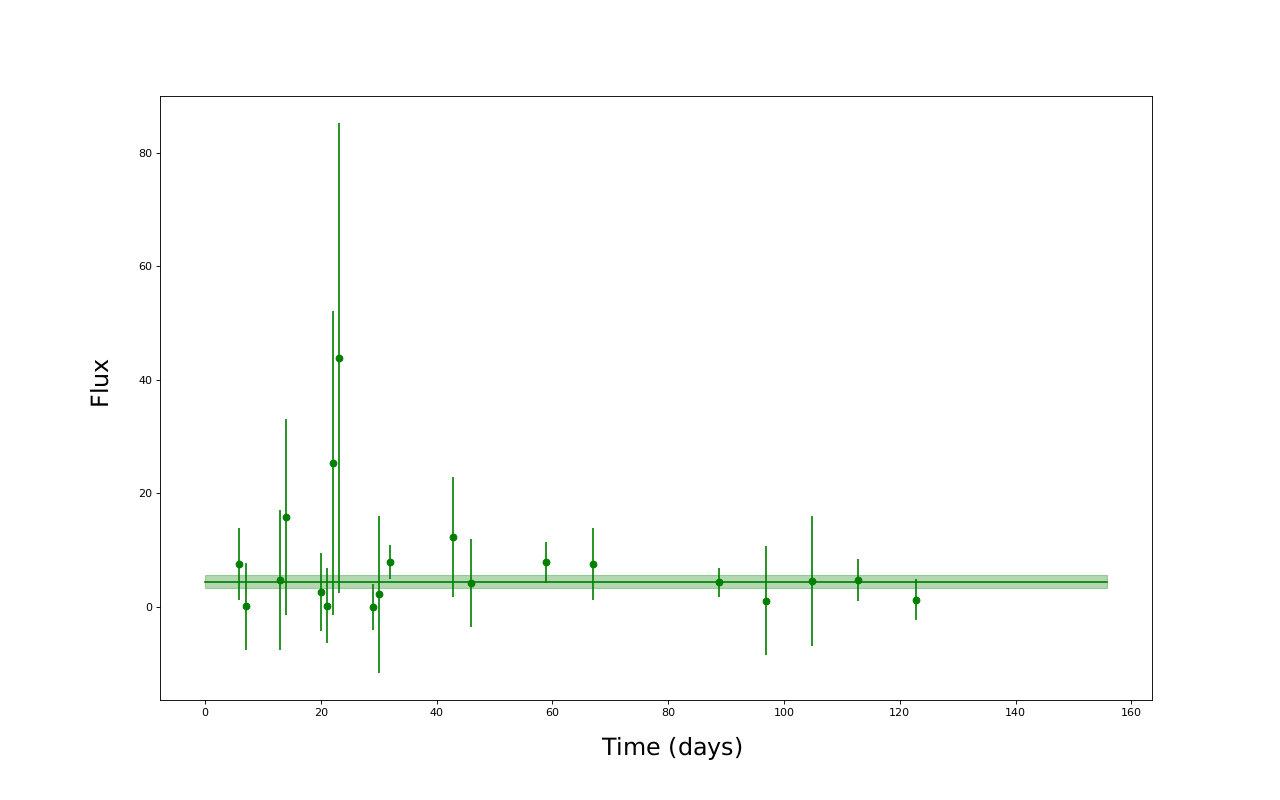
\includegraphics[width=15cm]{Ex_reta.png}
		\caption{Exemplo da interpolação não condizente com a realidade.}
		\label{fig:ExReto}
	\end{figure}
	
	\section{Delimitação}
	
	Todos os dados utilizados tanto neste trabalho quanto no artigo \cite{lochner}, foram extraídos da base de dados oferecida pelo desafio \citet{challenge}. A base de dados é de domínio público e pode ser obtida no {LINK DO DOWNLOAD}.
	
	Devido a granularidade dos dados brutos, é necessário um pré-tratamento visando buscar apenas os dados que iremos utilizar. Esse pré-tratamento foi aproveitado do \textit{pipeline} do Instituto de Física da UFRJ (\textbf{IF-UFRJ}), cujo processo visa ler os arquivos de texto transformando cada informação em uma chave de dicionário. 
	
	Ao fim do uso da seleção de dados citada acima, obtivemos valores em forma de dicionários em Python para cada objeto astronômico. Esses dicionários serão os \textbf{Dados Brutos} no escopo deste trabalho.   
	
	\section{Objetivos}
	\label{sec:Obj}
	
	O objetivo do trabalho é otimizar determinados pontos do \textit{pipeline} utilizado atualmente, após um estudo inicial ter sido feito para identificar pontos frágeis ou passíveis de melhoras.
	
	Esses pontos são apresentados e justificados a seguir, criando as três vertentes do trabalho
	
	\begin{itemize}
		\item Processo Gaussiano
		\item Aprendizagem Profunda
		\item Tratamento de \textit{Outliers}		
	\end{itemize}
	
		\subsection{Processo Gaussiano \textit{Gaussian Process}}
		
		O Processo Gaussiano, é a primeira parte do tratamento de dados após a transformação dos dados brutos em dicionários de Python. Iremos abordar esse procedimento no \autoref{chap:GP}.
		
		Cada objeto astronômico irá possuir uma quantidade de pontos que representam a intensidade do fluxo de luz captado em determinado dia, bem como a incerteza desse valor. Assim, buscamos fazer uma interpolação para obter um gráfico que passe por determinados pontos. 
		
		O objetivo ao abordar esse ponto é consertar interpolações que não condizem com a interpretação física, como pode ser vista na figura \ref{fig:ExReto}.
		
		\subsection{Aprendizagem Profunda}		

		A Aprendizagem Profunda (\textit{Deep Learning} ou \textbf{DL}) vêm sendo um advento utilizado recentemente para aprimorar alguns algoritmos de Aprendizagem de Máquina (\textit{Machine Learning} ou \textbf{ML}). 
		
		A ideia de aplicar DL nesse problema veio a partir da análise do \textit{pipeline} inicial (visto na seção \ref{sec:prob}). Tendo em vista que o mesmo possui diversas partes entre os dados brutos e algoritmo de RF, buscamos aplicar DL esperando obter um \textit{pipeline} mais simples, possuindo apenas uma etapa entre os dados brutos e o algoritmo de classificação.
		
		Em diversos outros casos na literatura, como identificação de sons ou imagens, houveram melhorias significativas ao reduzir o número de etapas envolvendo processamento de sinais (wavelets) ou redução de componentes (PCA) em troca do uso de DL. 
		
		A segunda motivação para a aplicação de DL veio do artigo da \citet{lochner}, onde ela menciona possíveis aplicações no escopo do problema.
		
		Assim, foi decidido aplicar algoritmos de DL após a primeira parte do tratamento de dados, visando manter uma simplicidade ao longo do \textit{pipeline}. Estabelecendo assim, apenas a etapa do GP entre os dados brutos e o algoritmo de classificação. O detalhamento desse procedimento encontra-se no \autoref{chap:DL}.

		\subsection{Tratamento de \textit{Outliers}}
		
		O último objetivo para buscar melhorias no algoritmo é o tratamento de pontos cuja incerteza é muito alta ou cujos valores são fora do esperado, pontos com essas características são conhecidos na literatura como \textit{outliers}.
		
		Analisando alguns dados brutos, observamos pontos cuja incerteza mostra-se mais de 100\% maior do que a própria curva (ponto mais a esquerda da figura \ref{fig:ExOutlierStd}) e também pontos que encontram-se completamente fora da curva interpolada \ref{fig:ExOutlier}.
		
		As etapas do tratamento encontram-se descritas no \autoref{chap:Out}.
		
		\newpage
		
		\begin{figure}[h!]
			\centering
			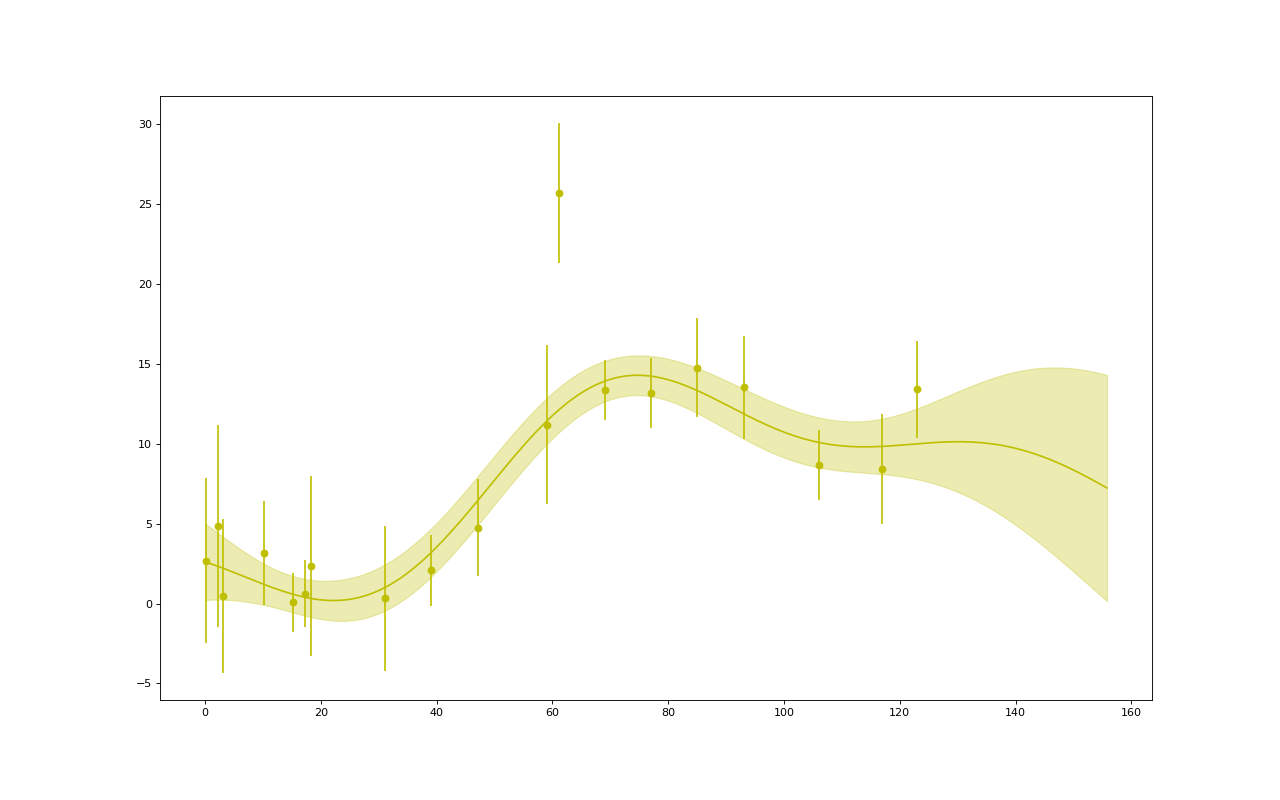
\includegraphics[width=15cm]{OutPoint.png}
			\caption{Exemplo de \textit{outlier}. Gráfico Fluxo $ \times $ Tempo (dias).}
			\label{fig:ExOutlier}
		\end{figure}
	
		\begin{figure}[h!]
		\centering
		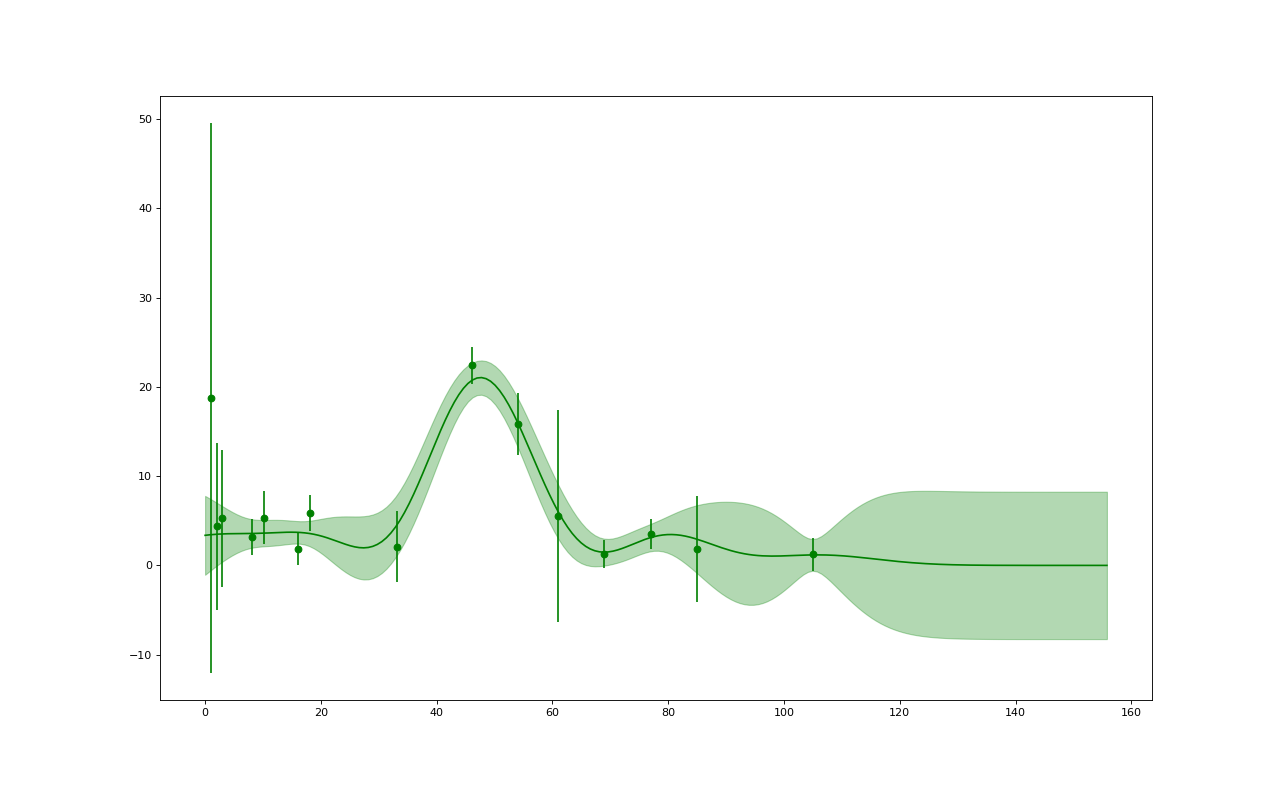
\includegraphics[width=15cm]{OutStd.png}
		\caption{Exemplo de ponto com incerteza 3 vezes maior que o pico da curva. Gráfico Fluxo $ \times $ Tempo (dias).}
		\label{fig:ExOutlierStd}
		\end{figure}
	

		
		\newpage

	\section{Metodologia}
	
	Devido ao código de pré-processamento do IF-UFRJ estar escrito em Python, todo o trabalho também foi escrito na mesma linguagem. Outro ponto para a escolha da linguagem foi a facilidade que a mesma possui para realizar experimentos através da plataforma \textit{Jupyter}, além da grande quantidade de bibliotecas de ciências de dados e suporte para desenvolver algoritmos de ML. 
	
	As principais bibliotecas utilizadas no contexto de tratamento de dados foram \textit{Pandas} e \textit{Numpy}. Já para a aplicação dos métodos as bibliotecas mais importantes foram \textit{scikit-learn}, \textit{Keras} e \textit{PyMC3}.
	
	A entrada dos modelos sempre serão os dicionários gerados a partir dos dados brutos após o pré-processamento do IF-UFRJ. Assim, pôde-se  filtrar com maior facilidade as propriedades desejadas para cada uma das três vertentes do trabalho. 

	Cada uma dessas vertentes possuiu um trabalho específico e isolado para poder melhor averiguar suas mudanças posteriormente. Em outras palavras, a cada mudança realizada houve a comparação direta com os resultados do \textit{pipeline} original, para poder avaliar especificamente a eficiência e melhora dessa mudança.
	
	Por se tratar de um algoritmo de classificação, a saída do nosso modelo será booleana e classificará se um objeto astronômico é ou não do tipo IA. Entretanto, nos dados brutos, as classes são divididas em 8 tipos de objetos: \textit{IA, IB, IBC, IC, II, IIL, IIN} e \textit{IIP}.
	
	É importante ressaltar também que para validar os modelos do projeto, foi usado o método \textit{K-fold}. Todavia, este trabalho se diferenciou da divisão clássica presente na literatura, que é uma divisão de 80\% dos dados para treinamento e 20\% para o teste dos modelos. Neste trabalho foram utilizados apenas 1100 objetos para treino dentre 21316 objetos totais. A justificativa é a limitação física das amostras.
	
	Por fim, as mudanças foram verificadas através de \textbf{Matrizes de Confusão} (\textit{Confusion Matrices} ou \textbf{CM}) ou através de métodos de \textit{score} da biblioteca \textit{scikit-learn}.
	
	Como última observação, a fim de estudos posteriores fora do escopo do projeto, todo o código desenvolvido encontra-se disponível em um repositório público do \textit{GitHub}. E nele foram feitas classificações envolvendo os 8 tipos de objetos, além de treinamentos adotando a proporção de 80\% para treino e 20\% para teste.
		
		
		
	\section{Descrição}
	No \autoref{chap:FundTeo}, iremos explicar os principais conceitos teóricos utilizados na aplicação do \textbf{Processo Gaussiano} e no \textbf{\textit{Deep Learning}}. Também serão levantados alguns conceitos não tão centrais do trabalho, mas de importância igualmente significativa.
	
	O \autoref{chap:ModeloAtual} será destinado para detalhar especificamente cada etapa do \textit{pipeline} atual, assim como uma breve menção a maneira na qual os dados brutos são tratados.
	
	Os capítulos 4, 5 e 6 serão destinados à explicação dos objetivos citados na seção \ref{sec:Obj}, assim como os resultados das mudanças que os mesmos causaram, buscando averiguar a eficiência de aplicação ou explicar possíveis erros.
	
	No \autoref{chap:Result} serão apresentados os resultados como um todo, seguidos de análises dos métodos através uma perspectiva global do projeto, diferentemente de como será nos capítulos anteriores, nos quais teremos uma visão específica para cada objetivo.
	
	Por fim, no \autoref{chap:Concl} tiraremos as conclusões finais do projeto e serão apresentadas sugestões de trabalhos futuros junto as limitações e possíveis soluções encontradas.
	
	\newpage
	
  \chapter{Fundamentos Teóricos}
  \label{chap:FundTeo}
  
 	\section{Processo Gaussiano \textit{Gaussian Process}}
 	
 	\section{Rede Neural Convolucional}
  
 	\section{Demais Conceitos}
 	
 		Conceitos menos usados ao longo do \textit{pipeline}, estão brevemente explicados a seguir.
 		
 		\subsection{Análise de Componentes Principais}
 		
 		\subsection{Transformadas de \textit{Wavelet}}
 		
  		\subsection{Validação Cruzada}
	\newpage
  \chapter{Modelo Atual}
  \label{chap:ModeloAtual}  		
  
  Neste capítulo iremos detalhar o modelo atual utilizado para estudos cosmológicos do IF-UFRJ.


	\section{Pré-processamento dos Dados Brutos}
	
	Como pode ser visto na figura \ref{fig:RawData}, os dados brutos chegam da seguinte forma para o pré-processamento.
	
	
	\begin{figure}[ht]
		\centering
		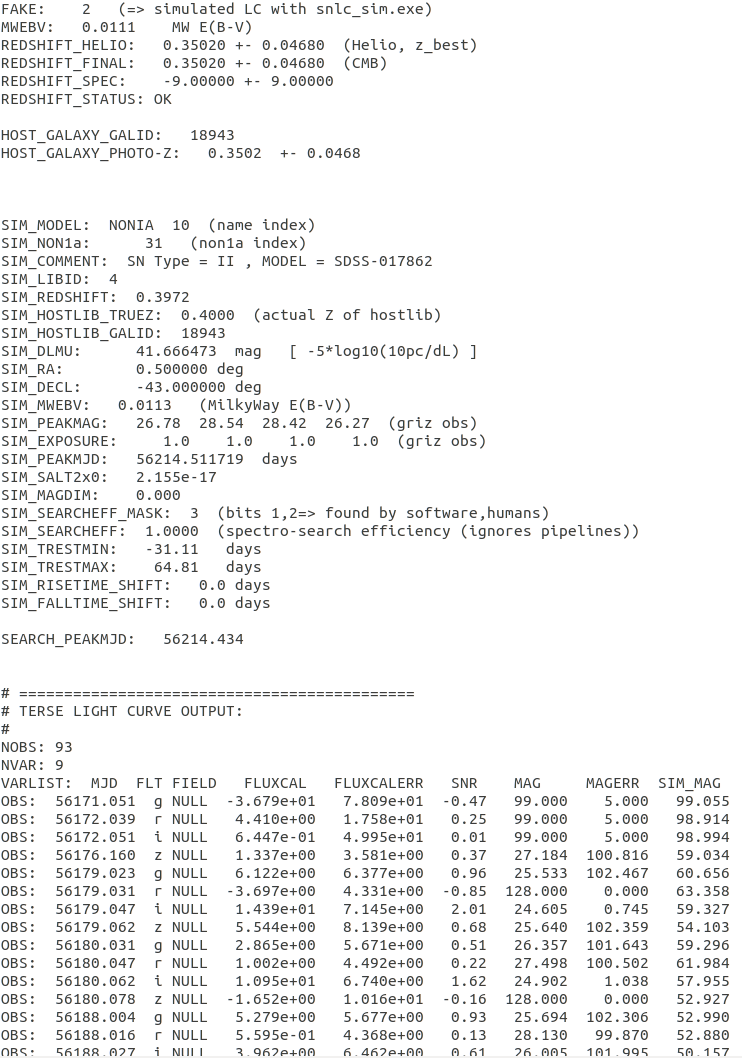
\includegraphics[width=9cm]{raw_dat.png}
		\caption{Arquivo \textit{.txt} a ser lido pelos arquivos de pré-processamento.}
		\label{fig:RawData}
	\end{figure}
	
	Através dos arquivos de pré-tratamento iremos obter todas essas informações em forma de dicionário, entretanto apenas as seguintes serão utilizadas durante o projeto.
	
	\begin{itemize}
		\item \textbf{SN TYPE} : Informa o tipo de supernova
		\item  \textbf{TERSE LIGHT CURVE OUTPUT} : Informa os pontos de observações obtidos. Será nosso \textit{Data Frame}. 
		\begin{itemize}
			\item \textbf{MJD} : O momento em que a observação foi obtida. A medida está descrita em dias do calendário Juliano.
			\item \textbf{FLT} : O filtro em que a observação foi obtida, pois cada observação é obtida a partir de um determinado espectro de luz. 
			\item  \textbf{FLUXCAL} : O valor do fluxo de luz obtido naquela observação.
			\item  \textbf{FLUXCALERR} : O valor do erro do fluxo de luz obtido naquela observação.
		\end{itemize}
	\end{itemize}

	Em relação ao \textbf{MJD}, vale ressaltar que é um método usado na astronomia para contar os dias sequencialmente, começando em uma data arbitrária no passado. Neste projeto, essas datas serão normalizadas, tendo como 0 o menor valor do MJD para que nosso eixo das abscissas tenha sempre início em 0.

	Em relação ao \textbf{FLT}, cada objeto astronômico é visto através de 4 filtros de luz diferentes, obtendo assim 4 curvas de luz para cada um deles. Para efeitos de aprendizagem de máquina, cada objeto possuirá 4 \textit{data frames}, um para cada filtro, e posteriormente essas propriedades serão convertidas em \textit{features} de cada objeto.
	
	A figura \ref{fig:ExFiltro} ilustra as 4 curvas de luz para o mesmo objeto.
	
	\begin{figure*}
		\centering
		\begin{subfigure}[b]{0.475\textwidth}
			\centering
			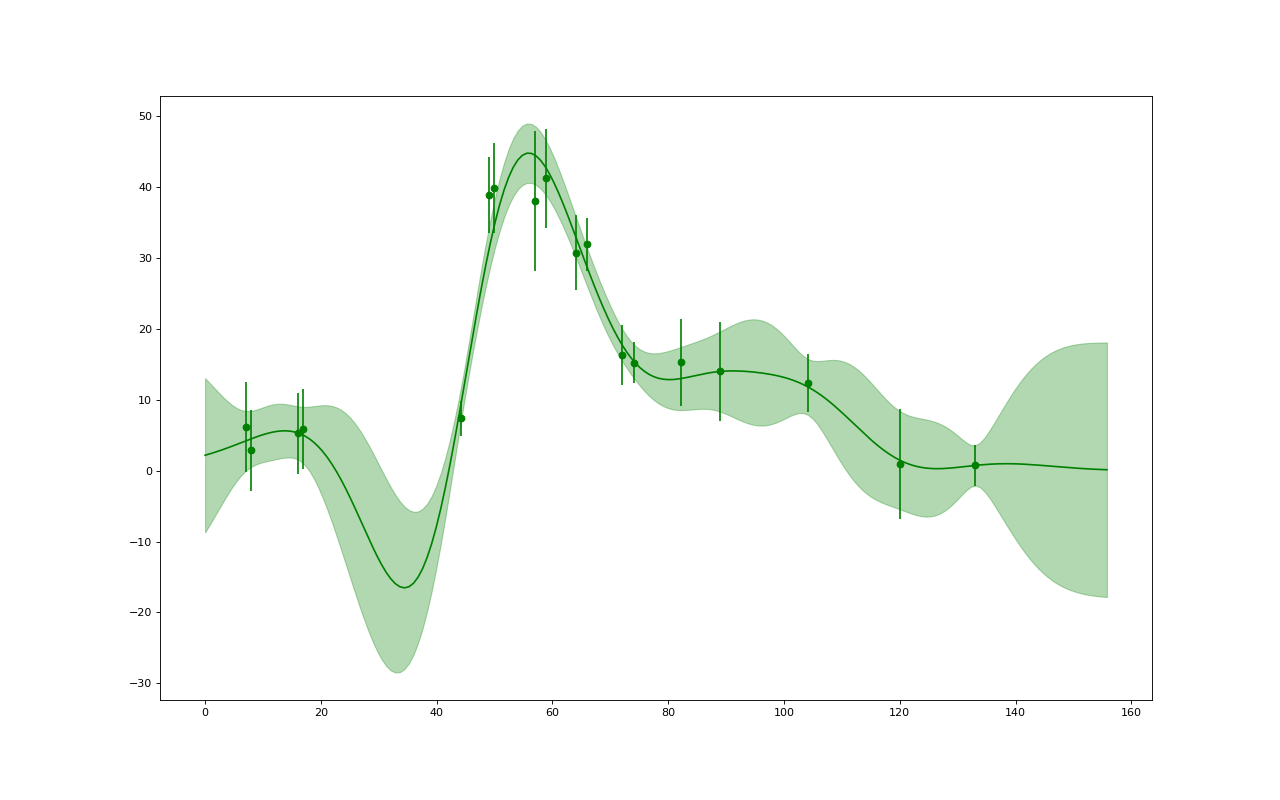
\includegraphics[width=\textwidth]{SN000017_II_desg.png}
			\caption[]%
			{{\small Filtro \textit{desg}}}    
			\label{fig:mean and std of net14}
		\end{subfigure}
		\hfill
		\begin{subfigure}[b]{0.475\textwidth}  
			\centering 
			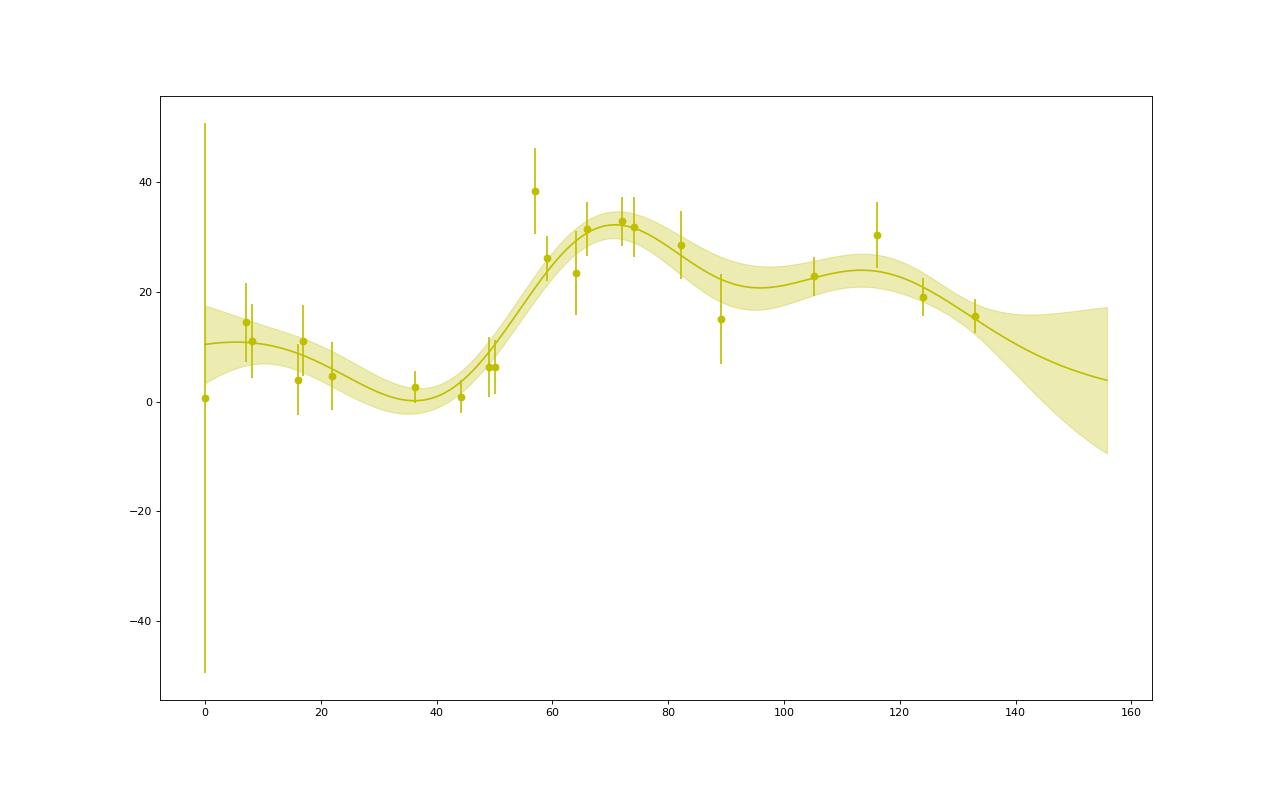
\includegraphics[width=\textwidth]{SN000017_II_desi.png}
			\caption[]%
			{{\small Filtro \textit{desi}}}    
			\label{fig:mean and std of net24}
		\end{subfigure}
		\vskip\baselineskip
		\begin{subfigure}[b]{0.475\textwidth}   
			\centering 
			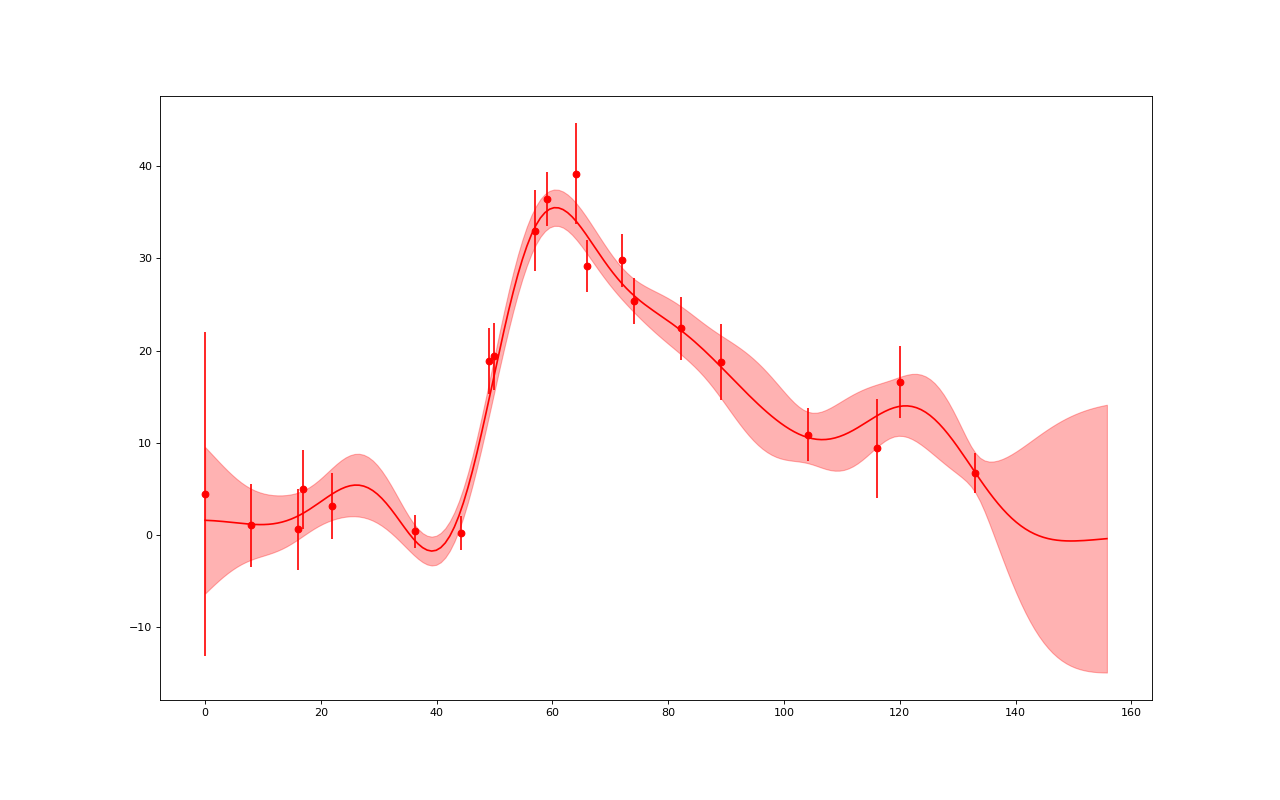
\includegraphics[width=\textwidth]{SN000017_II_desr.png}
			\caption[]%
			{{\small Filtro \textit{desr}}}    
			\label{fig:mean and std of net34}
		\end{subfigure}
		\quad
		\begin{subfigure}[b]{0.475\textwidth}   
			\centering 
			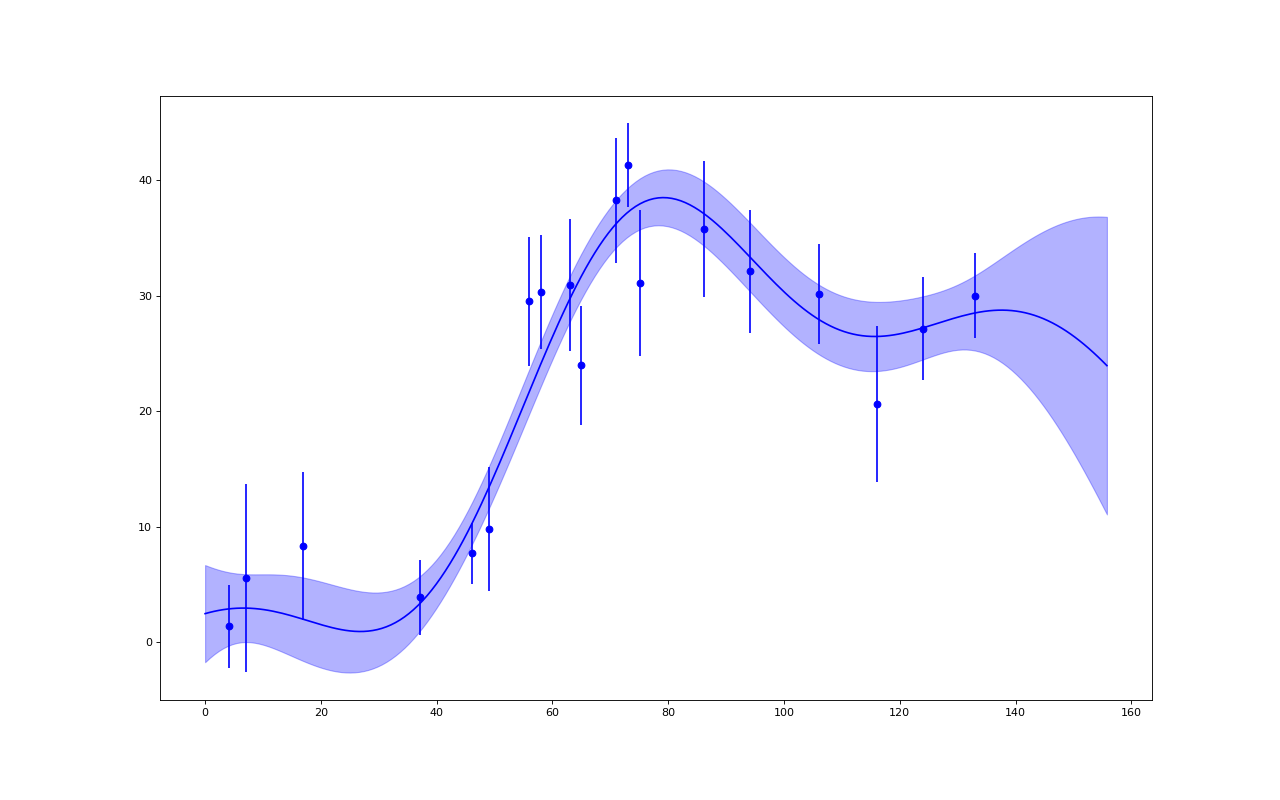
\includegraphics[width=\textwidth]{SN000017_II_desz.png}
			\caption[]%
			{{\small Filtro \textit{desz}}}    
			\label{fig:mean and std of net44}
		\end{subfigure}
		\caption[ Exemplo de 4 curvas de luz de um mesmo objeto, uma para cada filtro. Gráfico Fluxo $ \times $ Tempo (dias). ]
		{\small Exemplo de 4 curvas de luz de um mesmo objeto, uma para cada filtro. Gráfico Fluxo $ \times $ Tempo (dias).} 
		\label{fig:ExFiltro}
	\end{figure*}
	
	\section{\textit{Pipeline} Atual}
	
	A partir do pré-processamento explicado na seção anterior, o \textit{pipeline} atual irá dispor destes dados para realizar as etapas do processo de classificação.
	
	Inicialmente ele irá separar os dados do \textit{Terse Light Curve Output} pelos filtros e irá criar 4 \textit{dataframes} possuindo 3 \textit{features} cada, são eles: \textbf{MJD}, \textbf{FLUXCAL} e \textbf{FLUXCALERR}. \ref{fig:ImgDFMarc}
	
	\newpage
  \chapter{Tratamento de \textit{Outliers}}
  \label{chap:Out}
 	
 	\section{Estratégias Utilizadas}  	
 		
 	\section{Resultados e comparações}
	\newpage 		
  \chapter{Rede Neural Convolucional}
  \label{chap:DL}
 	A ideia foi blablabla usar deep learning, vimos exemplos das roupas, e colocamos la
 	deixamos a princípio o pipeline do Marcelo
 	 	
 	 \section{Geração de Imagens e Parâmetros}  	
 		Os parâmetros na hora de gerar as imagens e o PQ
 	\section{Escolhas de Redes Neurais}  	
 		escolhemos 2CNN pra fazer por isso e por aquilo
 	
 	\section{Resultados e comparações}
	\newpage
  \chapter{Interpolação através de Processo Gaussiano}
  \label{chap:GP}
  
	\section{Escolha da Biblioteca}
		
	\section{Aleatoriedades e \textit{Random Seeds}}
			
	\section{\textit{Kernel Functions}}
			
	\section{Demais Observações}
			Valor negativo e Mean function, erro grande, melhor overfittado que underfitado
			
	\section{Resultados das Interpolações}
		
	\section{Identificação e Justificativa do Erro}
	\newpage 
  \chapter{Resultados e Discussões}
  \label{chap:Result}
	\newpage
  \chapter{Conclusões}
  \label{chap:Concl}
	\section{Conclusões Finais} 	  
		
			Falar que o Algoritmo de hoje já é bem robusto
		
	\section{Trabalhos Futuros} 
		
			Falar de consertar o Erro e pah
		  

  \backmatter
  \bibliographystyle{coppe-unsrt}
  \bibliography{example}

  \appendix
  \chapter{Algumas Demonstrações}
\end{document}
%% 
%%
%% End of file `example.tex'.
